\section{Conformer: Atención Aumentada con Convolución}
\label{sec:annex-17}

\subsection{Resumen Ejecutivo}

El bloque Conformer \citep{Gulati2020} es el mezclador de secuencia aumentado con convolución del conjunto de herramientas, expuesto como \texttt{conformer\_attn}. Conserva el campo receptivo global de la atención de producto punto escalada y añade una rama de convolución depthwise que modela estructura local de banda estrecha---el sesgo inductivo que necesita el reconocimiento de voz y que la atención pura no aporta. El bloque intercala atención multi-cabeza (MHSA) con codificación posicional sinusoidal relativa entre dos capas feed-forward de medio paso estilo Macaron \citep{Lu2019}, e inserta el módulo de convolución entre la atención y la segunda FFN. En la receta de referencia alcanza $1.9\%$/$3.9\%$ WER en LibriSpeech \emph{test-clean}/\emph{test-other} sin modelo de lenguaje externo (Conformer-L, 118.8M parámetros), y es el mezclador recomendado para la clase de modelo de audio del Anexo~\ref{sec:annex-18}. El conjunto de herramientas ejecuta ambas capas feed-forward a paso completo (la variante ``full-step'' de la Tabla~5 del paper) y deja que la capa exterior posea la segunda; la Tabla~\ref{tab:conformer-mapping} lista las desviaciones.

El mezclador está disponible en todas las clases de modelo: encoder de texto, decoder causal (donde el padding depthwise se desplaza para seguir siendo seguro en streaming), Vision Transformer y \texttt{frankenstein\_audio}. Como el bloque vive dentro de \texttt{HybridLayer}, compone con los 45 mezcladores, las 6 normas, las 4 estrategias de residual, MoE, Mixture-of-Depths, mHC, AttnRes, BitNet y las 23 familias de optimizadores.

\subsection{Conformer: Atención Aumentada con Convolución}

\begin{figure}[H]
\centering
\fitfigure{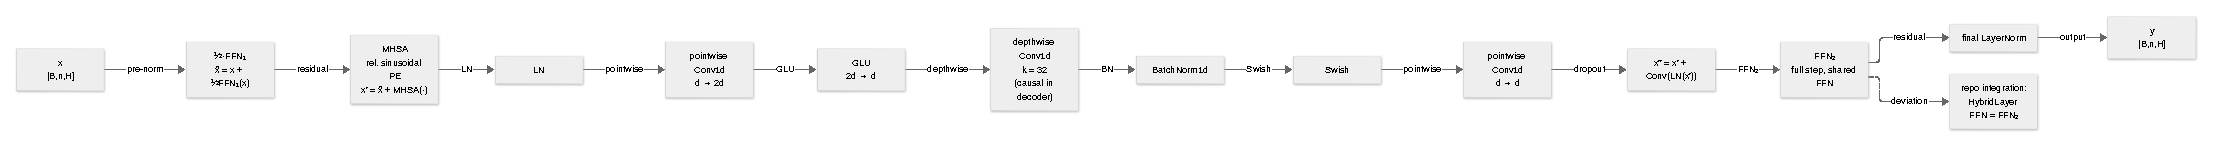
\includegraphics{../paper/figures/mixers/conformer.pdf}}
\caption{Flujo de datos del bloque Conformer: una capa feed-forward de medio paso Macaron, atención multi-cabeza con codificación posicional sinusoidal relativa, el módulo de convolución (pointwise $\to$ GLU $\to$ depthwise $\to$ BatchNorm $\to$ Swish $\to$ pointwise) y la segunda capa feed-forward seguida de la LayerNorm final. En este conjunto de herramientas la FFN compartida de \texttt{HybridLayer} ocupa la ranura $\mathrm{FFN}_2$ con un paso residual completo (anotación punteada).}
\label{fig:mixer-conformer}
\end{figure}

\subsubsection{Formulación Matemática}

Para una entrada de bloque $x \in \mathbb{R}^{B \times n \times d}$, el bloque de referencia de la Fig.~1 de \citet{Gulati2020} es
\begin{align}
\tilde{x} &= x + \tfrac{1}{2}\,\mathrm{FFN}_1\big(\mathrm{LN}(x)\big), \label{eq:conformer-ffn1}\\
x' &= \tilde{x} + \mathrm{MHSA}\big(\mathrm{LN}(\tilde{x})\big), \label{eq:conformer-mhsa}\\
x'' &= x' + \mathrm{Conv}\big(\mathrm{LN}(x')\big), \label{eq:conformer-conv}\\
y &= \mathrm{LN}\Big(x'' + \tfrac{1}{2}\,\mathrm{FFN}_2\big(x''\big)\Big). \label{eq:conformer-ffn2}
\end{align}
Los dos términos feed-forward llevan el coeficiente de \emph{medio paso} de Macaron: cada uno aporta la mitad de una actualización residual completa, uno antes y otro después del par atención--convolución.

\paragraph{Módulo feed-forward.} Con ancho oculto $d_{ff}$,
\begin{equation}
\mathrm{FFN}(x) = W_2\,\mathrm{Dropout}\big(\mathrm{Swish}(W_1\,\mathrm{LN}(x) + b_1)\big) + b_2,
\qquad
\mathrm{Swish}(a) = a\,\sigma(a),
\label{eq:conformer-ffn}
\end{equation}
donde $W_1 \in \mathbb{R}^{d_{ff} \times d}$, $W_2 \in \mathbb{R}^{d \times d_{ff}}$ y $\sigma$ es la sigmoide logística. El paper usa $d_{ff} = 4d$.

\paragraph{Atención multi-cabeza con codificación posicional relativa.} Las consultas, claves y valores son proyecciones lineales de la entrada normalizada del bloque, $Q = \mathrm{LN}(\tilde{x})W_Q$, $K = \mathrm{LN}(\tilde{x})W_K$, $V = \mathrm{LN}(\tilde{x})W_V$, divididas en $H$ cabezas de ancho $d_h = d/H$. Siguiendo el esquema relativo de Transformer-XL \citep{Dai2019}, la puntuación de la consulta $i$ contra la clave $j$ suma una función sinusoidal del \emph{desplazamiento} $i-j$ en lugar de una posición absoluta:
\begin{equation}
e_{ij} = q_i^{\top} k_j + (q_i + v)^{\top} R_{i-j},
\qquad
A_{ij} = \operatorname{softmax}_j\!\Big(\frac{e_{ij}}{\sqrt{d_h}}\Big),
\qquad
O = A V W_O,
\label{eq:conformer-relpe}
\end{equation}
con $v$ un vector de sesgo aprendido y, para $m = 0, \dots, d_h/2 - 1$,
\begin{equation}
R_{\delta,\,2m} = \sin\!\big(\delta\,/\,10000^{2m/d_h}\big),
\qquad
R_{\delta,\,2m+1} = \cos\!\big(\delta\,/\,10000^{2m/d_h}\big).
\label{eq:conformer-sinusoid}
\end{equation}
Como la codificación depende solo de $\delta = i-j$, el bloque generaliza entre longitudes de utterance. El conjunto de herramientas canaliza la información posicional por la maquinaria de todo el modelo que usan los demás mezcladores: \texttt{model.positional\_encoding} (RoPE por defecto) se aplica a $Q/K$, y \texttt{conformer\_attn\_use\_pe} (\texttt{true} por defecto) permite que una capa lo omita. El esquema sinusoidal relativo del paper se aproxima mejor con \texttt{sinusoidal\_rotary} (frecuencias sinusoidales aplicadas como rotación sobre $Q/K$, relativo por construcción); \texttt{alibi}/\texttt{bam} aportan un sesgo de distancia en lugar de una rotación. No se implementa un módulo sinusoidal relativo dedicado estilo Transformer-XL. En modo decoder la matriz de puntuaciones recibe la máscara causal habitual antes del softmax, y se usa la ruta de softmax fijo del Anexo~\ref{sec:fixed-implementation} cuando \texttt{numerics.fixed\_softmax} está habilitado.

\paragraph{Módulo de convolución.} El módulo aplica una convolución depthwise con compuerta sobre el eje temporal:
\begin{align}
h &= \mathrm{LN}(x'), \\
[u,\, g] &= \mathrm{Conv1d}_{d \to 2d}(h), \qquad
\tilde{h} = u \odot \sigma(g), \label{eq:conformer-glu}\\
z_t &= \sum_{k=0}^{K-1} w_k\, \tilde{h}_{t + k - \lfloor K/2 \rfloor}, \label{eq:conformer-depthwise}\\
c &= \mathrm{Dropout}\Big(\mathrm{Conv1d}_{d \to d}\big(\mathrm{Swish}(\mathrm{BN}(z))\big)\Big), \label{eq:conformer-conv-out}
\end{align}
donde $\odot$ es el producto elemento a elemento (una GLU que reduce los $2d$ canales a $d$), $w \in \mathbb{R}^{K}$ es el kernel depthwise y $\mathrm{BN}$ normaliza cada canal sobre los ejes de batch y tiempo,
\begin{equation}
\mathrm{BN}(z)_{b,t,c} = \gamma_c\,\frac{z_{b,t,c} - \mu_c}{\sqrt{\sigma_c^2 + \epsilon}} + \beta_c .
\label{eq:conformer-bn}
\end{equation}
En modo decoder la suma de la Ecuación~\ref{eq:conformer-depthwise} se desplaza a $z_t = \sum_{k=0}^{K-1} w_k \tilde{h}_{t-K+1+k}$, de modo que ninguna trama futura entra en la convolución; los modos encoder y ViT conservan el padding simétrico ``same'' del paper.

\subsubsection{Pseudocódigo Algorítmico}

\begin{algorithm}[H]
\caption{Bloque Conformer (\texttt{conformer\_attn})}
\begin{algorithmic}[1]
\Require entrada de bloque $x \in \mathbb{R}^{B \times n \times d}$, kernel $K=32$, cabezas $H$, bandera Macaron, modo
\Ensure delta de bloque $\Delta$ tal que $x + \Delta$ entra en la $\mathrm{norm}_2 + \mathrm{FFN}_2$ exterior
\State $\tilde{x} \gets x + \mathrm{FFN}_1(\mathrm{LN}(x))$ \Comment{FFN$_1$ Macaron ($\tfrac12$ en el paper)}
\State $Q, K_{proj}, V \gets \mathrm{LN}(\tilde{x})W_Q,\ \mathrm{LN}(\tilde{x})W_K,\ \mathrm{LN}(\tilde{x})W_V$
\State $e_{ij} \gets q_i^{\top}k_j + (q_i + v)^{\top}R_{i-j}$ \Comment{PE sinusoidal relativa, Ec.~\ref{eq:conformer-relpe}}
\If{modo $=$ decoder}
    \State $e_{ij} \gets -\infty$ para $j > i$ \Comment{máscara causal}
\EndIf
\State $x' \gets \tilde{x} + \mathrm{softmax}(e/\sqrt{d_h})\,V\,W_O$
\State $h \gets \mathrm{LN}(x')$
\State $[u, g] \gets \mathrm{Conv1d}_{d \to 2d}(h)$; \quad $\tilde{h} \gets u \odot \sigma(g)$ \Comment{GLU}
\State $z \gets \mathrm{DepthwiseConv1d}_{K}(\tilde{h})$ \Comment{desplazamiento causal en modo decoder}
\State $c \gets \mathrm{Dropout}(\mathrm{Conv1d}_{d \to d}(\mathrm{Swish}(\mathrm{BN}(z))))$
\State $x'' \gets x' + c$
\State \Return $x''$ \Comment{\texttt{HybridLayer} añade $\mathrm{FFN}_2$ y la LN final}
\end{algorithmic}
\end{algorithm}

\subsubsection{Mapeo de Implementación y Desviaciones}

La Tabla~\ref{tab:conformer-mapping} mapea el bloque del paper sobre el conjunto de herramientas. Las desviaciones sustantivas son los dos escalados residuales y la segunda capa feed-forward: el paper conserva ambos coeficientes $\tfrac12$ de Macaron y envuelve la $\mathrm{FFN}_2$ en el bloque, mientras que \texttt{conformer\_attn} usa pasos completos y devuelve el estado tras el módulo de convolución, dejando que el \texttt{HybridLayer} exterior aplique su $\mathrm{norm}_2 + \mathrm{FFN}$ compartida (también a paso completo). La descomposición es deliberada: mantiene disponibles para la segunda FFN el enrutamiento MoE, Mixture-of-Depths, los flujos mHC/Hyperloop, AttnRes, la fusión FlashNorm, las proyecciones BitNet y el enrutamiento de optimizadores por grupo de parámetros, nada de lo cual sobreviviría a una FFN privada dentro del mezclador.

\begin{table}[H]
\centering
\small
\begin{tabularx}{0.95\linewidth}{L{3.6cm}L{4.4cm}X}
\toprule
\textbf{Componente del paper} & \textbf{Implementación en el toolkit} & \textbf{Notas} \\
\midrule
$\tfrac{1}{2}\mathrm{FFN}_1$ (pre-norm) & FFN privada dentro de \texttt{ConformerAttention}; Swish; residual a paso completo & \texttt{conformer.macaron: true} (por defecto); el coeficiente $\tfrac12$ del paper se omite; deshabilitarla deja solo atención $+$ convolución \\
MHSA, PE sinusoidal relativa & proyecciones propias $q/k/v/out$; PE de todo el modelo vía \texttt{conformer\_attn\_use\_pe} (\texttt{true} por defecto) & la sinusoidal relativa del paper $\approx$ \texttt{sinusoidal\_rotary}; sin módulo Transformer-XL dedicado (RoPE es el valor por defecto del modelo) \\
Módulo de convolución & LN $\to$ pointwise $\to$ GLU $\to$ depthwise $\to$ BN $\to$ Swish $\to$ pointwise $\to$ dropout & \texttt{conformer.kernel\_size} (32), \texttt{conformer.conv\_norm} (\texttt{batch}/\texttt{group}/\texttt{layer}) \\
$\tfrac{1}{2}\mathrm{FFN}_2$ a medio paso & $\mathrm{norm}_2 + \mathrm{FFN}$ de \texttt{HybridLayer}, paso completo & justificado por la Tabla~5 de \citet{Gulati2020}: $1.9/4.4$ vs.\ $1.9/4.5$ WER dev (ambos coeficientes omitidos) \\
LayerNorm final & norma final de \texttt{HybridLayer} & idéntica a la de cualquier otro mezclador \\
Submuestreo convolucional $4\times$ & frontend de \texttt{frankenstein\_audio} & Anexo~\ref{sec:annex-18}; texto y ViT usan sus propios embeddings \\
Dropout ($p=0.1$) & \texttt{model.dims.dropout} & global, por bloque \\
\bottomrule
\end{tabularx}
\caption{Mapeo de implementación del bloque Conformer. Las desviaciones son los escalados Macaron $\tfrac12$ omitidos, la segunda FFN (aportada por la capa exterior a paso completo) y el cableado de la codificación posicional.}
\label{tab:conformer-mapping}
\end{table}

\paragraph{Por qué la FFN a paso completo es segura.} Omitir el $\tfrac12$ de Macaron cambia la escala residual de cada rama, no la forma expresiva del bloque: la variante de paso completo es exactamente la que \citet{Gulati2020} ablacionan en su Tabla~5, donde mueve el WER dev-clean/dev-other de $1.9/4.4$ (medio paso) a $1.9/4.5$ (paso completo), es decir, una décima. El conjunto de herramientas usa pasos completos en ambas capas feed-forward; la primera permanece privada en el mezclador y la segunda es la compartida, lo que preserva la composabilidad descrita arriba.

\subsection{Ablaciones Publicadas}

La Tabla~\ref{tab:conformer-ablations} resume las ablaciones que motivan la configuración por defecto. Los valores son los reportados por \citet{Gulati2020}; el orden cualitativo es lo que codifican los valores por defecto.

\begin{table}[H]
\centering
\small
\begin{tabularx}{0.95\linewidth}{L{3.7cm}L{4.0cm}X}
\toprule
\textbf{Ablación} & \textbf{Configuraciones comparadas} & \textbf{Resultado reportado} \\
\midrule
Módulo de convolución (Tabla~3) & presente vs.\ eliminado & la mayor degradación individual del bloque al eliminarlo; la rama local es portante, no decorativa \\
Par FFN Macaron (Tabla~3) & $\tfrac{1}{2}\mathrm{FFN}_1 + \tfrac{1}{2}\mathrm{FFN}_2$ vs.\ una FFN & eliminar el par cuesta aproximadamente $0.2$ dev-clean / $0.5$ dev-other WER \\
Medio vs.\ paso completo (Tabla~5) & residuales $\tfrac{1}{2}$ vs.\ completos & $1.9/4.4$ vs.\ $1.9/4.5$ WER dev: como máximo $0.1$ punto \\
Tamaño de kernel (Tabla~7) & $K \in \{3, 7, 17, 32, 65\}$ & $K = 32$ es el mejor; kernels pequeños subajustan el contexto local, $K = 65$ añade costo sin ganancia \\
Ubicación de la convolución & tras MHSA, antes de $\mathrm{FFN}_2$ & se conserva el orden de referencia; mover la rama no lo mejora \\
\bottomrule
\end{tabularx}
\caption{Ablaciones del Conformer y los valores por defecto que justifican (\texttt{kernel\_size: 32}, \texttt{macaron: true}, $\mathrm{FFN}_2$ compartida a paso completo).}
\label{tab:conformer-ablations}
\end{table}

\subsection{Reutilización de la Infraestructura Existente}

Como \texttt{ConformerAttention} devuelve un delta y hereda el constructor \texttt{mixer(config, pos\_encoder=...)}, toda la pila se reutiliza sin casos especiales:

\begin{itemize}[leftmargin=*]
    \item \textbf{Clases de modelo:} encoder de texto (\texttt{mlm}/\texttt{sbert}/\texttt{text\_classification}), decoder causal (\texttt{causal\_lm}), Vision Transformer (\texttt{patch\_prediction}/\texttt{classification}/\texttt{segmentation}) y \texttt{frankenstein\_audio} (\texttt{asr}, \texttt{audio\_classification}).
    \item \textbf{Normalización:} las 6 variantes, incluida pRMSNorm y la fusión FlashNorm en $\mathrm{norm}_1$/$\mathrm{norm}_2$; el módulo de convolución conserva su BatchNorm salvo que \texttt{conformer.conv\_norm} seleccione group o layer normalization.
    \item \textbf{Enrutamiento y residuales:} MoE, Mixture-of-Depths, mHC, Hyperloop, AttnRes y las proyecciones ternarias BitNet (la FFN privada y las proyecciones de la convolución son compatibles con BitLinear).
    \item \textbf{Optimizadores:} las 23 familias con prefijos por grupo; los parámetros del mezclador, incluido el kernel depthwise y las normas de la convolución, se enrutan al grupo \texttt{attention}.
    \item \textbf{Caché KV:} \texttt{conformer\_attn} se registra como \emph{no} cacheable (\texttt{supported=False}), porque el estado de la convolución depthwise y las estadísticas de BatchNorm deberían acarrearse entre pasos. \texttt{generate()} cae a la ruta de recómputo completo, que es exacta.
\end{itemize}

\subsection{Cuándo Usarlo}

\begin{itemize}[leftmargin=*]
    \item \textbf{Voz:} mezclador por defecto para \texttt{asr} y \texttt{audio\_classification}; con tramas de 40\,ms tras el submuestreo $4\times$, el kernel de 32 abarca $\sim$1.28\,s de contexto, aproximadamente el ancho de una secuencia de fonos.
    \item \textbf{Texto y visión:} sustituto sólido de \texttt{standard\_attn} cuando los datos tienen estructura local (modelos a nivel de carácter, código, OCR, secuencias de parches); cuesta una convolución depthwise y dos normas extra por capa frente a un bloque de atención plano.
    \item \textbf{Decodificación en streaming:} usable en \texttt{mode: decoder} con padding convolucional causal, pero sin la caché incremental del Anexo~\ref{sec:annex-kv-cache}; la recurrencia depthwise es la pieza que falta.
\end{itemize}
